\chapter{Rekursive Datentypen und Strukturelle Rekursion}
\section{Listen}
Mit strukturen können Datenobjekte mit einer festen Zahl von Daten gespeichert werden. Häufig wissen wir jedoch nicht, aus wie vielen Datenelementen eine Datenstruktur besteht.
%%%%%%%%%%%%%%%%%%%%%%%%%%%%%%%%%%%%%%%%%%%
Oder die struktur der Daten ist rekursiv
%???? KEINE AHNUNG WAS MIT DEM LETZTEN SATZ GEMEINT IST!!!
Mit rekursiven Datentypen können auch beliebig große Datenobjekte strukturiert abgespeichert werden. Die Idee davon ist die Folgende: Ein Element der Datenstruktur speichert (direkt oder indirekt) ein Exemplar der Datenstruktur. Dies nennt man dann eine \textit{rekursive Datenstruktur}. Um eine \uline{endliche} Datenstruktur zu bekommen benötigt man einen \textit{Rekursionsanker}. Diesen Rekursionsanker modellieren wir mit der Technik zu heterogenen Daten aus dem letzten Kapitel.

Eine Liste ist entweder die leere Liste the-emtpylst, oder (amke-lst s r), wobei s ein Wert ist und r eine Liste. Im folgenden sehen wir eine Modellierung von Listen mit Struktur.


\begin{lstlisting}{t03-prog1}
;; a list with 0 elements
;; (define list0 the-emptylst)
(define list0 empty)

;; a list with 1 element
;; (define list1 (make-lst 'a the-emptylst))
(define list1 (cons 'a empty))

;; a list with 2 elements
;; (define list2 (make-lst 'a
;;               (make-lst 'b the-emptylst)))
(define list2 (cons 'a (cons 'b empty)))

;; get the 2nd element from list2
;; (lst-first (lst-rest list2)) -> 'b
(first (rest list2)) ;; -> 'b
\end{lstlisting}

Listen sind ein wichtiger Datentyp, weshalb es einen eingebauten Datentyp existiert. Der Konstruktor \textit{cons} besitzt zwei argumente. cons entspricht unserem \textit{make-lst} Eigenbeispiel und steht wie es leicht zu vermuten ist für \textit{cons}truktor. Zudem existiert eine leere Liste \textit{emtpy} die unserer leeren Liste \textit{the-emptylst} entspricht. Auf die Sektoren der Liste kann man mit \textit{first} und \textit{rest} zugreifen. Mit \textit greift man auf das erste Element und mit \textit{rest} auf den Rest der Liste zu. Zudem haben beide noch \textit{historische Namen} die da lauten \textit{car} für \textit{first} und \textit{cdr} für rest. Die Prädikate \textit{lst?} und \textit{emtpy?} entsprechen \textit{lst?} und \textit{emptylst?}.
\textit{lst?} checkt ob es eine Liste ist und \textit{emptylst?} ob die Liste leer ist. Im Folgenden nun ein Beispiel:


\begin{lstlisting}{t03-prog2}
; a list with 0 elements
;; (define list0 the-emptylst)
(define list0 empty)

;; a list with 1 element
;; (define list1 (make-lst 'a the-emptylst))
(define list1 (cons 'a empty))

;; a list with 2 elements
;; (define list2 (make-lst 'a
;;               (make-lst 'b the-emptylst)))
(define list2 (cons 'a (cons 'b empty)))

;; get the 2nd element from list2
;; (lst-first (lst-rest list2)) -> 'b
(first (rest list2)) ;; -> 'b
\end{lstlisting}

Wie sie sehen besteht der einzige Unterschied zwischen \textit{make-lst} und \textit{cons} darin, dass \textit{cons} als zweites argument \textit{empty} oder \textit{(cons ...)}. Zum Beispiel :

\begin{lstlisting}{t03-prog3}
(cons 1 2)
\end{lstlisting}
ist ein Fehler
\begin{lstlisting}{t03-prog3}
(make-lst 1 2)
\end{lstlisting}
aber nicht.\\
\textit{cons} verhindert also inkorrekte Nutzung der Prozedur. In anderen LISP-basierten Dialekten fehlt allerdings diese Überprüfung. \\\\
Eine bessere Emulation sähe wie folgt aus:

\begin{lstlisting}{t01-prog4}
(define-struct lst (first rest))
(define-struct emptylst ())
(define the-emptylst (make-emptylst))
(define (our-cons a-value a-list)
  (cond
    [(emptylst? a-list) (make-lst a-value a-list)]
    [(lst? a-list) (make-lst a-value a-list)]
    [else (error 'our-cons "list as second argument expected")]))
\end{lstlisting}
Dies kann aber nicht verhindern, dass man \textit{make-lst} direkt verwendet. Im folgenden noch einige visuelle Beispiele.

\begin{lstlisting}{t03-prog4}
(cons 'Mercury empty)
\end{lstlisting}
\\
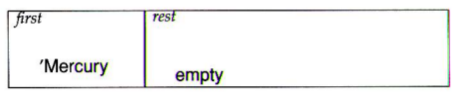
\includegraphics[height=2cm]{Bilder/T03_00.png}

\begin{lstlisting}{t03-prog4}
(cons 'Venus
    (cons 'Mercury empty))
\end{lstlisting}
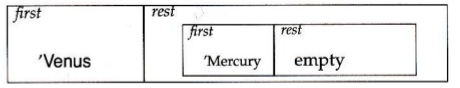
\includegraphics[height=2cm]{Bilder/T03_01.png}

\begin{lstlisting}
(cons 'Earth
  (cons 'Venus
	  (cons 'Mercury empty)))
\end{lstlisting}
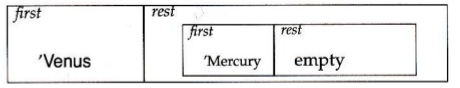
\includegraphics[height=2cm]{Bilder/T03_01.png}

In den folgenden Beispielen sehen wir: Listen speichern beliebige Datentypen, auch gemischte Daten.

\begin{lstlisting}{t03-prog5}
(cons 0
  (cons 1
    (cons 2
      (cons 3
        (cons 4
      	  (cons 5
            (cons 6
              (cons 7
                (cons 8
                  (cons 9 empty))))))))))
\end{lstlisting}

\begin{lstlisting}{t03-prog6}
(cons 'RobbyRound
  (cons 3
    (cons true empty)))
\end{lstlisting}
\section{Abgeschlossenheitseigenschaft}
Eine Operation zum Kombinieren von Daten besitzt die Abgeschlossenheitseigenschaft, wenn die Ergebnisse der Kombination von Datenobjekten wiederum mit der Operation kombiniert werden können. Betrachten wir hier \textit{cons} als Beispiel.
